\documentclass[11pt,a4paper]{article}
\usepackage[T1]{fontenc}
\usepackage{lmodern}
\usepackage[margin=20mm]{geometry}
\usepackage{amsmath,amssymb}
\usepackage{booktabs,graphicx,microtype,placeins}
\usepackage[numbers,sort&compress]{natbib}
\usepackage[hidelinks]{hyperref}

\newcommand{\Uniform}{UNIFORM}
\newcommand{\Tilt}{TILT}
\newcommand{\TiltName}{Linear Depth Tilt}
\newcommand{\FrozenProfile}{Frozen Offset Profile}
\newcommand{\Uprime}{\ensuremath{U'}}
\newcommand{\bten}{\texttt{b10}}
\newcommand{\bthirty}{\texttt{b30}}
\newcommand{\bfifty}{\texttt{b50}}
\newcommand{\bseventy}{\texttt{b70}}
\renewcommand{\topfraction}{0.9}
\renewcommand{\bottomfraction}{0.7}
\renewcommand{\textfraction}{0.08}
\renewcommand{\floatpagefraction}{0.65}
\setcounter{topnumber}{3}

\title{Allocating Channel Widths in CNN Folding:\\Parameter and MAC Budgets}
\author{}
\date{Internal review draft}
\hypersetup{pdftitle={Allocating Channel Widths in CNN Folding: Parameter and MAC Budgets}}

\begin{document}
\maketitle
\begin{abstract}
We study how to allocate a compression budget across coupled channel
groups in CNN folding. We hold the folding operator and batch-normalization
recalibration fixed, using training images for recalibration and no
post-compression weight fine-tuning. At matched parameter counts,
\TiltName{} (\Tilt{}) shifts retained width toward earlier groups and
improves top-1 over uniform folding in all 15 held-out settings, on all
four checkpoints in each. It uses
1.105--1.823 times as many multiply--accumulate operations (MACs). At
similar MAC counts, a wider uniform baseline with more parameters beats
\Tilt{} in 10 of 15 development settings. Under both uniform-folding caps,
we select the most accurate of 24 feasible profiles on CIFAR-100 development
data. The \FrozenProfile{} (L06) reuses the winning proposal's offsets
from uniform channel retention. At approximately 10\% parameter reduction,
it stays
within both caps and improves top-1 over uniform folding by 1.14
percentage points on Tiny ImageNet development data and 1.35 points on
2,000 ImageNetV2 images from the same 200 classes. Gains are positive on
each of the same four checkpoints in both samples. The paired 95\%
image-bootstrap interval for the ImageNetV2 gain is $[+0.700, +2.025]$
points, conditional on the four checkpoints.
\end{abstract}


\section{Introduction}
\label{sec:intro}

When folding a trained CNN, how should a fixed compression budget be
divided across the network? Folding reduces widths by merging similar
channels \citep{wang2025fold,saukh2026cut}. In a residual network, branches
that meet at an addition must agree in width, so the decision concerns
coupled groups of channels. The cost of retaining width also depends on
where it is retained: a convolution on a larger feature map uses more
multiply--accumulate operations (MACs) per weight. Two allocations with
the same parameter count can therefore have different MAC counts.

\citet[p.~13]{wang2025fold} leave per-layer sparsity optimization open.
Their study considers both uniform ratios and a setting that compresses
only the last two residual blocks \citep[pp.~11--12]{wang2025fold}.
\emph{Cut Less, Fold More} compares folding and magnitude pruning at the
same widths, using uniform per-layer ratios in its main CNN experiments
\citep[Figs.~1 and 8; Appendix~F.2]{saukh2026cut}. We ask how much accuracy
can be retained by changing the width allocation while keeping the
folding operator and batch-normalization (BN) recalibration fixed. BN
uses training images to re-estimate running statistics; there is no
post-compression weight fine-tuning.

We compare two profiles with uniform folding. \emph{\TiltName{}} (\Tilt{})
assigns smaller target channel reductions to earlier groups and larger ones
to later groups. It adapts a known linear rule
\citep{su2020random,huang2025atp} to match the uniform parameter count.
The \emph{\FrozenProfile{}} (L06) instead specifies a signed change to the
fraction of channels each group would retain under uniform folding. We
select the proposal by accuracy on CIFAR-100 development data from 24
candidates that meet both parameter and MAC caps. We freeze its offsets and
reuse them when projecting widths to other budgets.

\paragraph{Empirical contribution.} We measure the effect of a linear
depth profile at matched parameter counts and use cost controls to test
how the comparison changes when MACs are constrained. We then show that
the \FrozenProfile{} improves accuracy at mild compression under both
uniform-folding caps, on Tiny ImageNet development data and an external
ImageNetV2 sample from the same 200 classes.

\section{Related work}

\paragraph{Folding and channel merging.}
Model folding clusters and combines weights within a single network;
\citet{wang2025fold} study both data-based and data-free repair of affected
activation statistics. \citet{saukh2026cut} compare folding and magnitude
pruning as projections. Their reconstruction guarantee uses a one-rank
slack and concerns a weight-space approximation, so it does not specify a
network-wide allocation that maximizes post-recalibration top-1 accuracy.
Earlier approaches include Neuron Merging, which compensates for removed
channels in the weights of the next layer \citep{kim2020merging}, and
Iterative Feature Merging, which merges under a layer-local stopping
criterion and can leave different proportions of features across layers
\citep[Sec.~4 and Appendix~C]{chen2023ifm}. These are precedents for
post-training merging and for non-uniform compression.

\paragraph{Allocating compression.}
\citet[Appendix~C.2]{su2020random} compare decreasing keep-ratios, including
Linear Decay, with uniform and ascending allocations in unstructured
pruning followed by training. ATP uses an arithmetic progression of
layer sparsities and also reports experiments with vision models and
structured pruning \citep[Eq.~10 and Appendix~F]{huang2025atp}.
AutoDFP searches layerwise pruning ratios and channel reconstruction
coefficients; its uniform-vs-searched ablation is organized by nominal
parameter retention \citep[Table~I]{li2024autodfp}. In another compression
family, BALF allocates factorization ranks using activation distortion
under a global parameter or FLOP budget \citep[Sec.~4.3]{gonzalez2026balf}.
Our comparison varies coupled CNN widths within a fixed folding and BN
pipeline and examines the two network-wide costs separately and jointly.

\section{Method}
\label{sec:method}

\subsection{Channel groups, costs, and folding}

A channel group ties the producer and consumer axes that require a
common width, including axes coupled by residual additions. We use the
upstream group order, with 12 groups in ResNet18 and 13 in
PreActResNet18. Let $n_g$ be the original width of group $g$ and $k_g$ the
retained width. The vector $\mathbf k$ determines tensor shapes. The
parameter count $P(\mathbf k)$ includes all model parameters, including
BN affine parameters and biases, and excludes running-statistic buffers.
$M(\mathbf k)$ counts MACs per image for convolutional and linear layers
at the specified input size. For example, a convolution with output
spatial size $H\times W$, kernel size $h\times w$, and $q$ convolution
groups contributes $HW hw C_{\rm in} C_{\rm out}/q$ MACs. Bias additions,
normalization, and other operations are not included in $M$. We check the
costs of the rebuilt models; $M$ is an architecture cost, distinct from a
measurement of latency.

We use the upstream folding implementation of \citet{saukh2026cut}
(\href{https://github.com/osaukh/folding_as_projection/tree/694691556e8314a835178a741938dd3d4d80c171}{commit \texttt{6946915}}).
An adapter supplies explicit retained widths and preserves the classifier bias. The same
clustering and weight-merging procedure operates at the specified
$k_g$ for each allocation. Tiny ImageNet uses a torchvision ResNet18
with the $7\times7$ stride-two stem, max-pooling, and a 200-class head at
$64\times64$ input resolution. This uses the upstream operator on our
models and checkpoints rather than reproducing the upstream training
study.

\subsection{Uniform folding and Linear Depth Tilt}
\label{sec:tilt}

\Uniform{} (denoted $U$) specifies a common channel reduction before
integer rounding. For $G$ coupled groups and $g=0,\ldots,G-1$, the
\TiltName{} profile (denoted $T$) is based on
\begin{equation}
 p_g = \frac{2g}{G-1}-1,\qquad
 r_g(b,\alpha) = \operatorname{clip}(b+\alpha p_g, 0.10, 0.90),\qquad
 k_g(b) = \left\lfloor n_g\bigl(1-r_g(b,\alpha)\bigr)\right\rfloor .
 \label{eq:tilt}
\end{equation}
Here $r_g$ is the fraction of channels to remove, and $p_g$ indexes the
groups from early to late. With $\alpha=0$ the target is uniform. With
$\alpha>0$, the target reduction increases linearly from $b-\alpha$ to
$b+\alpha$ before clipping and rounding. This is the depth tilt: earlier
groups have lower target reductions than later groups. Before clipping,
Equation~\eqref{eq:tilt} is in the affine family of
ATP: with $g=i-1$ and $G=L$, setting $b=S$ and $\alpha=\beta(G-1)/2$
recovers its arithmetic progression \citep[Eq.~10]{huang2025atp}. In our
adaptation, $b$ is chosen against a cost of the rebuilt network, rather
than a mean of layer sparsities.

For a nominal parameter reduction $d\in\{0.30,0.50,0.70\}$, we first
find $U$ with $\alpha=0$ and parameter cap
$\operatorname{round}((1-d)P(\mathbf n))$. We then use $\alpha=0.30$ and
cap $P(U)$ for $T$. For both, 60 bisection steps choose $b$ on the feasible
side of the cap. For $T$ only, we increment one group at a time where
possible, never exceeding the cap or $\lfloor0.9n_g\rfloor$. The selected
increment gives the largest feasible $P$ and ties go to the lower group
index. The actual $P(T)$ lies in $[0.999P(U),P(U)]$ in all 15 held-out
settings (Table~\ref{tab:tilt-uniform}). Here and below, labels such as
\bfifty{} denote nominal parameter reductions of the reference, not
per-group channel reductions. We use the same width plans on development
and held-out splits without tuning $\alpha$ or widths on held-out data.

\subsection{Matching MACs and imposing both caps}
\label{sec:caps}

\paragraph{MAC-matched uniform control.} For the wider uniform profile
\Uprime{}, we choose a common channel reduction to approach $M(T)$ from
below. With integer widths, $M(\Uprime{})$ is within 2\% of $M(T)$ in each
setting. $P(\Uprime{})$ is free to differ. We compare all three profiles on
the same development images, reusing the $U$ and $T$ scores from the
development phase of the parameter-matched comparison. The profiles
start from the same checkpoints and use the same BN recalibration protocol.

\paragraph{Matching both costs to \Tilt{}.} We test four controls on
ResNet18 at \bfifty{} on CIFAR-10 and CIFAR-100 development data. The controls
start from fixed permutations of earlier \Tilt{} width deviations. To
derive the realized widths, we find a nearby continuous profile using a
least-squares distance in retained fractions $k_g/n_g$. For cost caps
$(C_P,C_M)$, the continuous targets are
$P=0.9995C_P$ and $M=0.9995C_M$. We use sequential least-squares programming,
round to integer widths, and if necessary deterministically correct at
most two groups. The final widths must spend $99.9$--$100\%$ of each cap
without exceeding either one. This fits a cost-constrained geometry; it
does not use accuracy as the projection objective. For these controls, the
caps are $P(T)$ and $M(T)$. The controls are adjusted profiles derived from
permutations, not exact permutations after projection.

\subsection{Frozen Offset Profile under joint parameter and MAC caps}
\label{sec:l06}

\paragraph{Constrained selection on development data.} We set the
caps to the realized parameter count $P(U)$ and MAC count $M(U)$ of uniform
folding at a nominal 50\% parameter reduction. Before scoring, we fix 24
distinct feasible profiles per dataset using the projection in
Section~\ref{sec:caps}: eight width exchanges within stages, four exchanges
across stages, and twelve proposals with random offsets in the retained
fractions. The ResNet18 width domain is
$\lfloor0.1n_g\rfloor\leq k_g\leq\lfloor0.9n_g\rfloor$. For every
candidate, both realized costs fall within 0.1\% of the respective caps
and do not exceed them.

Let $\mathcal K_{24}$ be this feasible pool for CIFAR-100 and let
$A_{\mathrm{dev},s}(\mathbf k)$ be development top-1 on checkpoint $s$
after folding to widths $\mathbf k$ and recalibrating BN. We select one
profile across all four checkpoints by solving
\begin{equation}
 \mathbf k^\star \in \operatorname*{arg\,max}_{\mathbf k\in\mathcal K_{24}}
   \frac{1}{4}\sum_{s=42}^{45} A_{\mathrm{dev},s}(\mathbf k).
 \label{eq:profile-selection}
\end{equation}
The winner, identified as L06 in the experiment records, comes from the
random-offset candidates. Uniform folding ($U$) and the original
\Tilt{} profile projected onto the same caps
($T_{\rm proj}$) are separate references. CIFAR-10 is a development
control and does not select the \FrozenProfile{} used in later evaluations.

\paragraph{Frozen offsets.} From the selected proposal, we retain the
original offsets in $k_g/n_g$ units (shown here in percentage points in
upstream group order):
\begin{equation}
 \mathbf o=(+2,-15,-14,+13,-1,-5,-6,+9,-12,-13,+17,-6).
 \label{eq:offsets}
\end{equation}
An offset of $-15$ percentage points proposes $55\%$ retention if
uniform folding would retain $70\%$. A positive offset proposes keeping
more channels. At a new budget, we add $n_g o_g/100$ to the uniform width
$k_g^U$, round to nearest (ties to even), and clip to the legal width
domain before projecting to the two caps. The offsets stay frozen while
the realized widths are fitted to the target costs. At \bfifty{} on the
CIFAR-100 reserve we reproduce the selected widths exactly; on Tiny
ImageNet we recalculate costs for its stem and input resolution.

\paragraph{Mild compression on Tiny ImageNet.} We evaluate the frozen
offsets at a nominal 10\% parameter reduction (\bten{}), using the
realized parameter and MAC counts of uniform folding at the same budget
as caps. On Tiny ImageNet, the previous upper bound
$\lfloor0.9n_g\rfloor$ would force at least a 19.21\% parameter reduction
and cannot reach the \bten{} cost window. We therefore allow $k_g\le n_g$
for the projection at this budget, with the same lower bound and both
cost checks. The final width vector in upstream order is
\[
 \mathbf k = (64,52,53,128,127,119,233,256,219,434,512,476).
\]
Four groups retain their original width. The external ImageNetV2
evaluation uses these exact widths without repeating profile selection
or projection.

\subsection{BN recalibration and fixed checkpoints}

We study existing ResNet18 checkpoints \citep{he2016resnet} for
CIFAR-10, CIFAR-100 \citep{krizhevsky2009cifar}, and Tiny ImageNet
\citep{stanfordTinyImageNet}, and PreActResNet18 checkpoints
\citep{he2016preact} for both CIFAR datasets. CIFAR inputs are
$32\times32$ and Tiny inputs are $64\times64$. The four source seeds
are 42--45 for each model--dataset pair. The full models were trained
from random initialization for 200 epochs using SGD (initial learning
rate 0.1, momentum 0.9, weight decay $5\times10^{-4}$, cosine scheduling)
with batches of 128 per independently trained model. Each folding
comparison starts from the same source checkpoint for all profiles.

The primary recalibration is A4096/CMA: reset the BN
\citep{ioffe2015bn} running statistics, then run 32 batches of 128 images
with cumulative moving average updates. A4096 is a fixed set of 4,096
images from the corresponding training split, with fixed crop and
horizontal-flip views and training normalization. No labels are used
for this pass. Only BN buffers change; the affine parameters and the
other weights are frozen. The same procedure is used for the full model
as a reference. We include the upstream \texttt{repair\_bn} pass from a
separate copy of the folded state as a secondary control where reported;
it is a statistics repair related to REPAIR \citep{jordan2023repair}.
These are data-calibrated, fine-tuning-free comparisons. Archived quality
runs used four RTX 2080 Ti GPUs, one paired seed per GPU, with deterministic
FP32 and TF32 disabled.

\section{Evaluation protocol}
\label{sec:evaluation}

\paragraph{Development and held-out data.} We compare the fixed $U$ and
$T$ profiles on the official CIFAR-10 and CIFAR-100 test sets and the
official Tiny ImageNet validation set, with 10,000 images in each. Tiny
validation had previously been inspected for input shapes but had not
been used to score a model. Before the held-out evaluation, we reproduced
the development scores and checked that the calibrated states were
identical across both phases. The MAC-matched uniform comparison, the
controls matched to \Tilt{} on both costs, profile selection, and the
mild-compression comparisons on Tiny ImageNet use development splits.
These contain 5,000 images for each CIFAR dataset and 10,000 for Tiny,
drawn from the respective official training partitions and separate from
training/calibration images.

\paragraph{Further evaluations of the \FrozenProfile{}.} On CIFAR-100, we
evaluate the frozen proposal on a separate 5,000-image reserve set aside
from the official training partition before source model training,
disjoint from development and calibration images. We use the same
checkpoints as for profile selection. We transfer the proposal to Tiny
ImageNet, which did not participate in profile selection. At larger
parameter reductions we reuse the official Tiny ImageNet validation
images from the held-out $U/T$ comparison. The mild-compression
evaluation instead uses the 10,000-image Tiny ImageNet development split.
These scores refer to distinct sampling roles.

\paragraph{External ImageNetV2 sample.} The ImageNetV2 MatchedFrequency
release \texttt{imagenetv2-b-33} \citep{recht2019imagenetv2} is restricted
to all 200 class identifiers used in Tiny ImageNet. We verify the label
mapping against the release metadata and compare candidate images
against the 110,000 Tiny training, development, and official validation
images using an exact RGB and perceptual hash screen. No duplicates are
flagged by that screen, leaving 2,000 images, ten per class. We resize the
whole RGB image bilinearly to $64\times64$ after EXIF orientation and
apply the same normalization as in the Tiny ImageNet development
evaluation, without augmentation. Before scoring on ImageNetV2, we
verified that all 12 post-CMA model states (three variants per checkpoint)
and their costs matched those used for mild compression on the Tiny
ImageNet development split. BN continues to use Tiny training images,
without adapting to ImageNetV2.

\paragraph{Paired outcomes and uncertainty.} For each setting we subtract
accuracies within a checkpoint on the same images and then average across
checkpoints. We report sample standard deviation (SD) of the paired
differences when given, and the number of strictly positive pairs. Loss to
the full model is its post-CMA accuracy minus that of the folded model.
Direction and magnitude thresholds are prespecified decision criteria;
the 15 cells of the held-out $U/T$ comparison reuse checkpoints and are
not 60 independent trials. For ImageNetV2, we estimate a paired percentile
interval by 10,000 bootstrap draws, resampling images within each class
and using identical image indices for all variants and checkpoints in
each draw. This measures image-sample variability conditional on the four
fixed checkpoints and the specified classes. We use the same bootstrap
design for the comparison of the \FrozenProfile{} with uniform folding at
\bfifty{} on the official Tiny ImageNet validation set.

\section{Results}
\label{sec:results}

\subsection{Allocation effect at matched parameter counts}

\Tilt{} improves CMA top-1 over \Uniform{} in all 15 settings
on the official CIFAR test sets and Tiny validation set, with positive
paired differences on all four checkpoints in every setting
(Figure~\ref{fig:matched-parameters}, Table~\ref{tab:tilt-uniform}). Mean
gains range from $+0.8100$ to $+22.7375$ percentage points (pp). A distinct magnitude
criterion of at least $2$ pp in the mean and at least three positive
pairs at \bfifty{} or \bseventy{} is met in 9 of 10 settings; the exception
is ResNet18/CIFAR-100 at \bfifty{} ($+1.3025$ pp). The effect on
ResNet18/CIFAR-100 at \bseventy{} is uneven, with differences of $+0.20$
and $+0.36$ pp on two of four checkpoints despite a $+2.0600$ pp mean.

\begin{figure}[htbp]
  \centering
  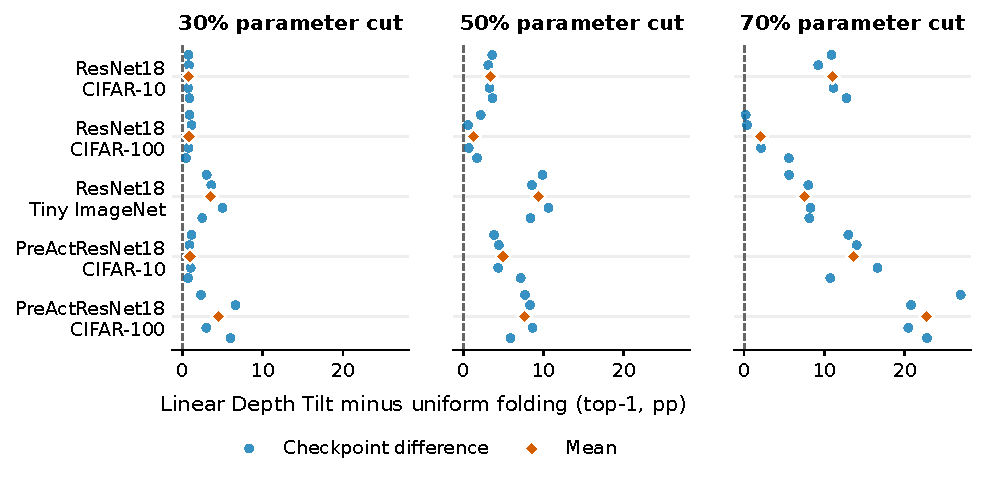
\includegraphics[width=\linewidth]{../experiments/2026-11-07_E035_ocena_niezalezna/figures/publikacja/e035_tilt_minus_uniform_en.pdf}
  \caption{\textbf{\TiltName{} (\Tilt{}) vs. uniform folding at matched
  parameter counts.} Each point is a within-checkpoint difference after CMA;
  diamonds are means over the four checkpoints. Budgets are nominal
  parameter reductions. CIFAR scores are from the official test splits;
  Tiny ImageNet uses the official validation split. The vertical line
  marks equal top-1.}
  \label{fig:matched-parameters}
\end{figure}
% Generated from the audited runs by paper/prepare_tables.py.
\begin{table}[tbp]
\centering
\small
\setlength{\tabcolsep}{5pt}
\caption{\textbf{Matched parameters.} Top-1 after CMA on the official CIFAR tests and Tiny ImageNet validation set. Budgets are nominal reductions in total parameters. $U$ is \Uniform{} and $T$ is \TiltName{} (\Tilt{}); the $T-U$ column gives the paired mean and sample SD across checkpoints, in percentage points (pp). The last column counts strictly positive differences.}
\label{tab:tilt-uniform}
\begin{tabular}{@{}llrrrrrr@{}}
\toprule
 &  &  & \multicolumn{3}{c}{Top-1 (\%)} &  &  \\
\cmidrule(lr){4-6}
Architecture & Dataset & $P$ cut & Full & $U$ & $T$ & $T-U$ (pp) & Positive \\
\midrule
ResNet18 & CIFAR-10 & 30\% & 94.8050 & 93.0400 & 93.8500 & $+0.8100\pm 0.0594$ & 4/4 \\
 &  & 50\% & 94.8050 & 89.2800 & 92.6925 & $+3.4125\pm 0.2564$ & 4/4 \\
 &  & 70\% & 94.8050 & 76.7925 & 87.7800 & $+10.9875\pm 1.4358$ & 4/4 \\
\addlinespace[2pt]
ResNet18 & CIFAR-100 & 30\% & 74.3725 & 65.7675 & 66.5950 & $+0.8275\pm 0.2863$ & 4/4 \\
 &  & 50\% & 74.3725 & 53.4275 & 54.7300 & $+1.3025\pm 0.7834$ & 4/4 \\
 &  & 70\% & 74.3725 & 30.6200 & 32.6800 & $+2.0600\pm 2.4948$ & 4/4 \\
\addlinespace[2pt]
ResNet18 & Tiny ImageNet & 30\% & 50.7775 & 34.5575 & 38.0950 & $+3.5375\pm 1.0847$ & 4/4 \\
 &  & 50\% & 50.7775 & 19.6400 & 29.0000 & $+9.3600\pm 1.0830$ & 4/4 \\
 &  & 70\% & 50.7775 & 8.3975 & 15.8800 & $+7.4825\pm 1.2595$ & 4/4 \\
\addlinespace[2pt]
PreActResNet18 & CIFAR-10 & 30\% & 94.9025 & 93.1275 & 94.0875 & $+0.9600\pm 0.1944$ & 4/4 \\
 &  & 50\% & 94.9025 & 88.5400 & 93.4900 & $+4.9500\pm 1.5034$ & 4/4 \\
 &  & 70\% & 94.9025 & 77.6875 & 91.2650 & $+13.5775\pm 2.4453$ & 4/4 \\
\addlinespace[2pt]
PreActResNet18 & CIFAR-100 & 30\% & 76.4700 & 66.4975 & 70.9850 & $+4.4875\pm 2.1362$ & 4/4 \\
 &  & 50\% & 76.4700 & 55.9050 & 63.5475 & $+7.6425\pm 1.2266$ & 4/4 \\
 &  & 70\% & 76.4700 & 23.0050 & 45.7425 & $+22.7375\pm 3.0018$ & 4/4 \\
\bottomrule
\end{tabular}
\end{table}


With the original \texttt{repair\_bn}, the directional criterion
(positive mean and at least three positive pairs) is met in 14 of 15
settings rather than 15. The exception is ResNet18/CIFAR-100 at
\bseventy{} (2/4). On that model and dataset the mean negative
log-likelihood after CMA is also higher for \Tilt{} at \bfifty{} and
\bseventy{}. Relative top-1 improvement does not imply high absolute
accuracy: at \bseventy{}, ResNet18/Tiny achieves 15.8800\% with \Tilt{}
versus 50.7775\% for the full model.

\subsection{Cost of the allocation gain}
\label{sec:allocation-cost}

\paragraph{Arithmetic and measured runtime.} Counting operations for the
parameter-matched width profiles gives $M(T)/M(U)=1.105$--$1.823$
(Table~\ref{tab:cost-controls}). Earlier feature maps have more spatial
positions, so retaining a wider channel group there can use more MACs
even if later layers shrink enough to offset its additional parameters.
We measured device-only forward passes on synthetic inputs, excluding
loading and host--device transfers. At batch size 128, the mean
throughput ratio of \Tilt{} to \Uniform{} ranges from 0.702 to 0.948
across settings. At batch size 1, mean latency ratios range from 0.965 to
1.046 (across-checkpoint SDs of ratios: 0.019--0.100). Those timings do
not establish equivalent latency or a consistent single-image latency
ordering. They are measurements on one hardware setup.

\paragraph{Uniform folding at comparable MACs.} On common development
images, \Uprime{} outperforms \Tilt{} in 10 of 15 settings. The advantage
of \Uprime{} reaches $23.69$ pp on ResNet18/CIFAR-100 at \bseventy{}.
Its parameter count is $1.10$--$1.82$ times that of \Tilt{}, even though
the MAC ratio $M(\Uprime{})/M(T)$ is between 0.985 and 0.999 after
rounding to three decimals. Figure~\ref{fig:comparable-macs} displays the same
development scores against both costs. Increasing uniform width changes
parameter capacity as well as MACs; the result limits the practical
claim about \Tilt{} at comparable MACs without isolating the role of
either cost in its gain at matched parameter counts.

\begin{figure}[htbp]
  \centering
  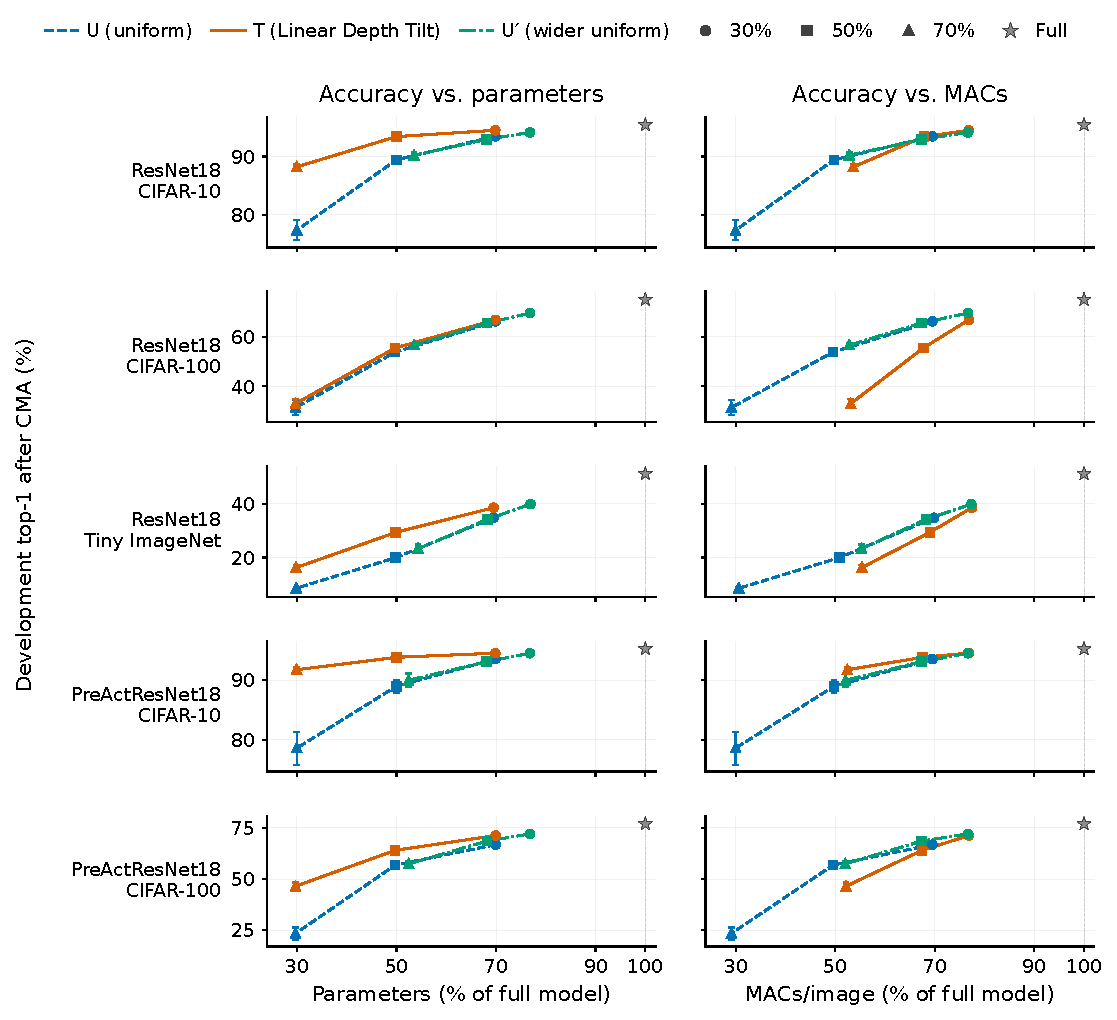
\includegraphics[width=\linewidth]{../experiments/2026-11-08_E037_kontrola_mac/figures/publikacja/e037_accuracy_cost_en.pdf}
  \caption{\textbf{Accuracy and cost on common development splits.}
  At comparable MACs, the wider uniform baseline \Uprime{} beats
  \TiltName{} in 10 of 15 settings and has more parameters. Rows are
  model--dataset pairs. Both columns show the same CMA top-1 scores,
  with axes showing actual parameters (left) or MACs per
  image (right) as percentages of the corresponding full model costs.
  Markers identify the nominal parameter cuts of $U$ and $T$, and the
  associated MAC targets of \Uprime{}. Points and bars are means and
  sample SD across four checkpoints. Within each row, the top-1 scale is
  shared; scales differ between rows.}
  \label{fig:comparable-macs}
\end{figure}
% Generated from the audited runs by paper/prepare_tables.py.
\begin{table}[tbp]
\centering
\small
\setlength{\tabcolsep}{3.5pt}
\caption{\textbf{Cost and accuracy on development data.} Top-1 uses the same development split and CMA protocol for uniform folding ($U$), \TiltName{} ($T$), and the wider uniform model $U'$. The anchor is the nominal parameter reduction of $U$ and $T$, not of $U'$. The $U'-T$ column is the mean paired difference; positive values favor $U'$. Section~\ref{sec:allocation-cost} summarizes forward-pass timing ratios.}
\label{tab:cost-controls}
\begin{tabular}{@{}llrrrrrrrr@{}}
\toprule
 &  &  & \multicolumn{3}{c}{Top-1 (\%)} &  & \multicolumn{3}{c}{Cost ratios} \\
\cmidrule(lr){4-6}\cmidrule(lr){8-10}
Architecture & Dataset & Anchor & $U$ & $T$ & $U'$ & $U'-T$ (pp) & \shortstack{MACs\\$T/U$} & \shortstack{Params.\\$U'/T$} & \shortstack{MACs\\$U'/T$} \\
\midrule
ResNet18 & CIFAR-10 & 30\% & 93.495 & 94.520 & 94.155 & $-0.365$ & 1.105 & 1.100 & 0.998 \\
 &  & 50\% & 89.435 & 93.430 & 92.955 & $-0.475$ & 1.364 & 1.363 & 0.992 \\
 &  & 70\% & 77.305 & 88.215 & 90.225 & $+2.010$ & 1.789 & 1.788 & 0.985 \\
\addlinespace[2pt]
ResNet18 & CIFAR-100 & 30\% & 66.340 & 66.960 & 69.670 & $+2.710$ & 1.105 & 1.100 & 0.998 \\
 &  & 50\% & 53.855 & 55.550 & 65.660 & $+10.110$ & 1.366 & 1.371 & 0.994 \\
 &  & 70\% & 31.400 & 33.020 & 56.710 & $+23.690$ & 1.823 & 1.804 & 0.995 \\
\addlinespace[2pt]
ResNet18 & Tiny ImageNet & 30\% & 34.807 & 38.587 & 39.913 & $+1.325$ & 1.109 & 1.106 & 0.998 \\
 &  & 50\% & 19.925 & 29.333 & 34.170 & $+4.837$ & 1.357 & 1.369 & 0.988 \\
 &  & 70\% & 8.433 & 16.180 & 23.240 & $+7.060$ & 1.806 & 1.821 & 0.999 \\
\addlinespace[2pt]
PreActResNet18 & CIFAR-10 & 30\% & 93.590 & 94.575 & 94.550 & $-0.025$ & 1.105 & 1.099 & 0.998 \\
 &  & 50\% & 88.995 & 93.875 & 93.135 & $-0.740$ & 1.358 & 1.363 & 0.996 \\
 &  & 70\% & 78.595 & 91.785 & 90.000 & $-1.785$ & 1.748 & 1.750 & 0.993 \\
\addlinespace[2pt]
PreActResNet18 & CIFAR-100 & 30\% & 66.870 & 71.305 & 72.120 & $+0.815$ & 1.105 & 1.099 & 0.998 \\
 &  & 50\% & 56.845 & 64.070 & 68.585 & $+4.515$ & 1.361 & 1.371 & 0.998 \\
 &  & 70\% & 23.425 & 46.520 & 57.460 & $+10.940$ & 1.790 & 1.766 & 0.998 \\
\bottomrule
\end{tabular}
\end{table}


\paragraph{Simultaneous matching to \Tilt{}.} With both costs
matched to \Tilt{}, its advantage over the mean of the four prespecified
alternative profiles is $+0.11250$ pp (2/4) on CIFAR-10 and $+2.10375$ pp
(4/4) on CIFAR-100 (Table~\ref{tab:dual-tilt}). One CIFAR-10 control
(104) beats \Tilt{} by $0.3850$ pp on average and wins on all four
checkpoints. On CIFAR-100, \Tilt{} beats even the strongest of the four
control means, by $0.8600$ pp. The combined directional criterion
requiring a positive mean and at least three positive pairs on each
dataset is not met. Tiny ImageNet was outside this pilot's scope. This
comparison separates the profile from increases in either static cost
for those controls; it does not establish that \Tilt{} generally wins
when both costs are matched.
% Generated from the audited runs by paper/prepare_tables.py.
\begin{table}[tbp]
\centering
\small
\setlength{\tabcolsep}{5pt}
\caption{\textbf{Both costs matched to \Tilt{}.} Four prespecified ResNet18 controls at the nominal 50\% parameter cut, each using 99.9--100\% of \Tilt{}'s parameters and MACs. $\bar C$ is the mean of the four controls within each checkpoint. The positive count refers to $T-\bar C$. The best control is identified descriptively by mean development top-1.}
\label{tab:dual-tilt}
\begin{tabular}{@{}lrrrrrr@{}}
\toprule
 & \multicolumn{2}{c}{Top-1 (\%)} &  &  &  &  \\
\cmidrule(lr){2-3}
Dataset & $T$ & $\bar C$ & $T-\bar C$ (pp) & Positive & Best control & $T-$best (pp) \\
\midrule
CIFAR-10 & 93.4300 & 93.31750 & $+0.11250\pm 0.2184$ & 2/4 & 104 & $-0.3850$ \\
CIFAR-100 & 55.5500 & 53.44625 & $+2.10375\pm 0.7602$ & 4/4 & 103 & $+0.8600$ \\
\bottomrule
\end{tabular}
\end{table}

\FloatBarrier

\subsection{Accuracy under both uniform-folding caps}

\paragraph{Profile selection.} At \bfifty{} on CIFAR-100 development
data, the profile selected by Equation~\eqref{eq:profile-selection}
improves top-1 over the stronger reference, $U$, by $1.175$ pp (3/4).
Only 5 of the 24 candidates beat $U$ on average, and the median contrast
to $U$ is $-1.265$ pp. This gain is measured on the split used for
selection. The remaining experiments assess the frozen
proposal outside the data used for that selection.

\paragraph{Mild compression on Tiny ImageNet development data.} The
\FrozenProfile{} at \bten{} has 10,104,855 parameters and 132,302,192 MACs
per image, below $U$ by 6,575 parameters and 34,004 MACs per image. These
counts are 10.41\% and 10.70\% lower than the full model, respectively.
We first reproduced the eight full-model and uniform-folding states and
scores previously obtained on this split. The \FrozenProfile{}
improves mean top-1 from 46.3625\% to 47.5050\%: $+1.1425$ pp (sample SD
$0.8820$ pp), with four positive pairs. The mean loss to the full model
falls from 4.8575 to 3.7150 pp (Table~\ref{tab:b10},
Figure~\ref{fig:b10}A). For context, \Uniform{} at a nominal
20\% parameter reduction loses 10.6400 pp on this same split.

\paragraph{External confirmation on ImageNetV2.} In the independent
image sample from the same 200 classes, \Uniform{} attains 26.9875\%
and the \FrozenProfile{} attains 28.3375\%. The gain of $+1.3500$ pp (sample SD 0.9704 pp)
is positive on all four checkpoints. The loss from the full model (30.3375\%)
decreases from 3.35 to 2.00 pp. The paired 95\% image-bootstrap interval
for the gain, $[+0.700,+2.025]$ pp, excludes zero (Figure~\ref{fig:b10}B).
The prespecified confirmation criterion (positive mean, at least three
positive pairs, and positive lower interval limit) is met. Each model has
the same parameter and MAC counts as in the evaluation on the Tiny
ImageNet development split (Table~\ref{tab:b10}). The interval pertains
to image variation at the fixed checkpoints, and the lower absolute
accuracy on ImageNetV2 also affects the full model.

\begin{figure}[htbp]
  \centering
  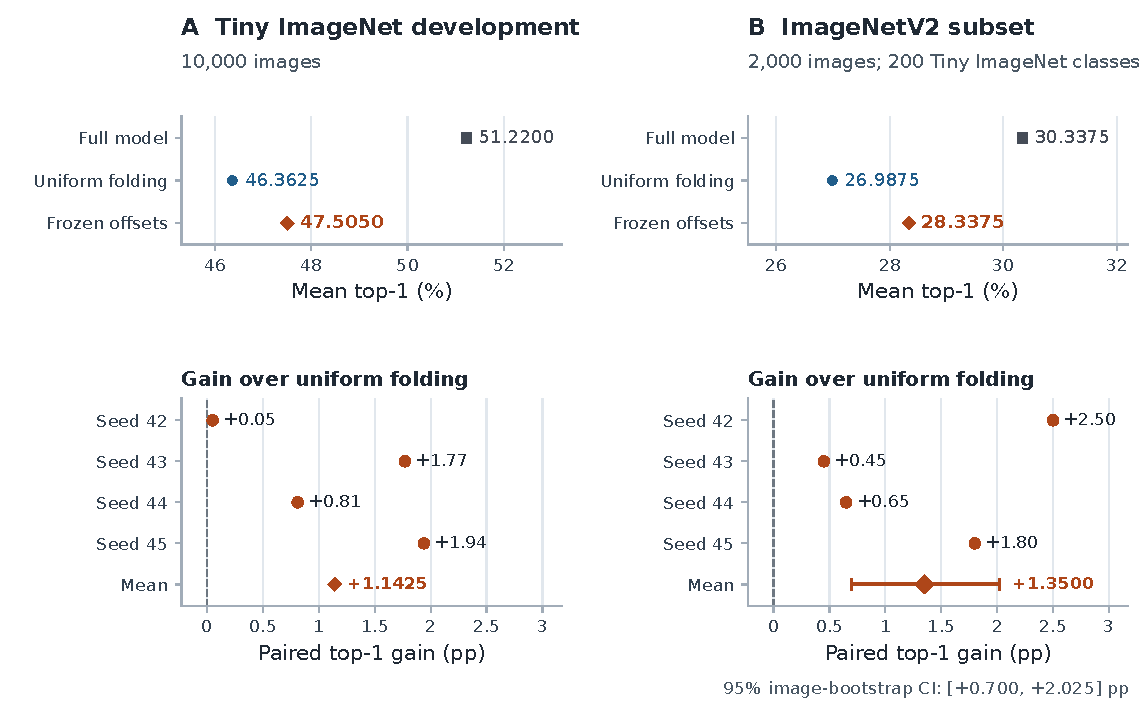
\includegraphics[width=\linewidth]{../experiments/2026-11-22_E047_l06_b10_imagenetv2/wykresy/20261122T053804Z_ae2dec73/b10_tiny_imagenetv2_en.pdf}
  \caption{\textbf{Accuracy gains under both uniform-folding caps.}
  A: Tiny ImageNet development split. B: external ImageNetV2
  MatchedFrequency sample restricted to the 200 Tiny ImageNet classes.
  Upper plots show mean post-CMA top-1 across the same four checkpoints
  with separate accuracy scales. Lower plots show the paired top-1 gains
  for the \FrozenProfile{} (L06, labeled ``Frozen offsets'') over uniform
  folding, with means marked by diamonds. The bar in B
  gives the paired 95\% image-bootstrap interval conditional on the four
  checkpoints. Table~\ref{tab:b10} gives the actual costs for both panels.}
  \label{fig:b10}
\end{figure}
% Generated from the audited runs by paper/prepare_tables.py.
\begin{table}[tbp]
\centering
\small
\setlength{\tabcolsep}{8pt}
\caption{\textbf{Mild compression under both uniform-folding caps.} Cost counts are identical across samples. For each checkpoint, top-1 loss is the full model's top-1 minus that of the specified model on the same images. Values are mean $\pm$ sample SD across four checkpoints after CMA. The ImageNetV2 sample is MatchedFrequency restricted to the 200 Tiny ImageNet classes.}
\label{tab:b10}
\begin{tabular}{@{}lrrrr@{}}
\toprule
Model & Parameters & MACs/image & Top-1 (\%) & Paired loss (pp) \\
\midrule
\multicolumn{5}{@{}l}{\textbf{Tiny ImageNet development split (10,000 images)}} \\
\addlinespace[2pt]
Full model & 11,279,112 & 148,148,224 & $51.2200\pm 0.1602$ & 0 \\
Uniform folding & 10,111,430 & 132,336,196 & $46.3625\pm 0.4687$ & $4.8575\pm 0.5309$ \\
Frozen Offset Profile & 10,104,855 & 132,302,192 & $47.5050\pm 0.4458$ & $3.7150\pm 0.5132$ \\
\midrule
\multicolumn{5}{@{}l}{\textbf{ImageNetV2 (2,000 images)}} \\
\addlinespace[2pt]
Full model & 11,279,112 & 148,148,224 & $30.3375\pm 0.3198$ & 0 \\
Uniform folding & 10,111,430 & 132,336,196 & $26.9875\pm 1.0711$ & $3.3500\pm 0.7853$ \\
Frozen Offset Profile & 10,104,855 & 132,302,192 & $28.3375\pm 0.2496$ & $2.0000\pm 0.2483$ \\
\bottomrule
\end{tabular}
\end{table}


\paragraph{Supporting results at larger cuts.} On the
CIFAR-100 reserve, the \FrozenProfile{} gains $+1.215$ pp (3/4) at \bfifty{} over $U$ and
$+1.065$ pp (4/4) over $T_{\rm proj}$. At \bthirty{}, the $+0.945$ pp gain
over $U$ (4/4) falls below the prespecified $+1.00$ pp practical threshold.
The profile remains 19.970 and 7.420 pp below the full model at the two budgets,
respectively. On the previously used official Tiny validation set, the
transferred profile gains $+2.100$ pp (4/4) at \bfifty{} and $+0.255$ pp (3/4)
at \bthirty{}. The 95\% paired image interval at \bfifty{} is
$[+1.67,+2.52]$ pp conditional on the four checkpoints, but the absolute
gap to the full model is still 29.0375 pp. These complementary evaluations
test the frozen offsets at larger cuts, with different roles for the
reserved CIFAR images and reused Tiny validation images.
\FloatBarrier

\section{Discussion and limitations}

Matching model size by parameter count can make a width allocation look
attractive while leaving it more expensive to execute. The comparison at
similar MACs (Figure~\ref{fig:comparable-macs}) shows why a uniform
baseline should also be sized for the computational budget of interest.
The mixed results for the controls matched to \Tilt{} on both costs
(Table~\ref{tab:dual-tilt}) show that controlling both counts does not
remove all allocation effects, but neither their direction nor size can
be inferred solely from a depth-dependent rule. The paired comparisons
with the \FrozenProfile{} provide an example in which width redistribution
improves top-1 under both uniform-folding caps.

The \FrozenProfile{} was selected using labeled development data. Its
optimality is limited to the 24 candidates and the selection setting.
The tests span two related residual architectures and four
checkpoints per setting. The ImageNetV2 evaluation changes the image
source for one model family and one mild budget; it does not add training
replicates or extend the class set. The different image distribution and
input preprocessing do not permit attributing the absolute accuracy gap
between sources to one cause. The image-level intervals do not capture uncertainty across
newly trained models, and development, reserve, reused validation, and
external evaluations should not be pooled as independent replications.

The reported resource caps constrain static counts. Even two networks
with nearly the same counts can have different activation shapes, peak
memory, or achieved latency. The device-only forward-pass measurements
cover one environment, not deployment performance, and the \bten{} study
does not measure a latency gain. Finally, larger relative gains at
aggressive cuts can coexist with substantial absolute errors. These results therefore
characterize controlled comparisons with a uniform folding baseline;
they do not rank whole compression pipelines or establish a universal
allocation rule.

\section{Conclusion}

With a fixed folding operator and data-based BN recalibration, reallocating
channel widths changes how much top-1 accuracy a compressed CNN retains.
The linear \Tilt{} profile consistently improves on \Uniform{} at
matched parameter counts while using more MACs, and does not consistently
beat a wider \Uniform{} at comparable MACs. Under both realized
uniform-folding caps at mild compression, the \FrozenProfile{} improves
top-1 by 1.1425 pp on Tiny development data and 1.3500 pp on the external
ImageNetV2 sample. The contrast between these findings motivates reporting
both costs when comparing folding allocations without weight fine-tuning.

\paragraph{Reproducibility.} The repository links the experiment identifiers
to frozen plans, run manifests, and audited CSV and JSON files. The tables
have machine-readable counterparts. The notes in \texttt{paper/README.md}
map claims to the archived results and document how to regenerate the
tables, figures, and PDF.

\begingroup
\small
\raggedright
\bibliographystyle{unsrtnat}
\bibliography{references}
\endgroup
\end{document}
